\section{Questions et réponses}
\subsection{Pattyn}
\subsubsection{Logique}
\begin{description}
	\item [Le réchauffement est plus fort en antarctique qu'en arctique. ]
	\color{cyan}Vrai\color{black}
	
	\item [Le réchauffement est plus fort au pole nord qu'au pole sud. ]
	\color{cyan}Faux\color{black}

	\item [Révolution Néolithique est le passage de chasse/pêche à l'agriculture. ]
	\color{cyan}Vrai\color{black}

	\item [Après l'ère Néolithique vient l'ère Anthropique. ]
	\color{cyan}Faux\color{black}

	\item [Après l'ère Paléolithique vient l'ère Néolithique. ]
	\color{cyan}Vrai\color{black}
\end{description}



\subsubsection{Pourquoi le réchauffement est plus élevé au pole ? Pourquoi il y a un réchauffement important en Antarctique ?}
\color{cyan}
À cause du vortex polaire qui se manifeste au-dessus des régions polaires au cours des hivers locaux. Il est plus important au pôle sud qu'au pole nord, l'Antarctique est donc le continent le plus froid du globe. C'est une circulation bien structurée des vents dans la stratosphère. Il empêche l'air stratosphérique au-dessus des régions polaires de se mélanger avec de l'air venant des moyennes latitudes.
\color{black}



\subsubsection{Classez les gaz à effet de serre selon leur importance.}
\color{cyan}
\begin{itemize}
	\item \textbf{$H_2O$} Vapeur d'eau ;
	\item \textbf{$CO_2$} Dioxyde de carbone ;
	\item \textbf{$CH_4$} Méthane ;
	\item \textbf{$CCI_2F_2$} Dichlorodifluorométhane (CFC-12) ;
	\item \textbf{$CHCIF_2$} Chlorodifluorométhane (HCFC-22) ;
	\item \textbf{$CF_4$} Tétrafluorométhane ;
	\item \textbf{$SF_6$} Hexafluorure de soufre.
\end{itemize}
\color{black}



\subsubsection{Cycle de formation du carbone à compléter}
\color{cyan}
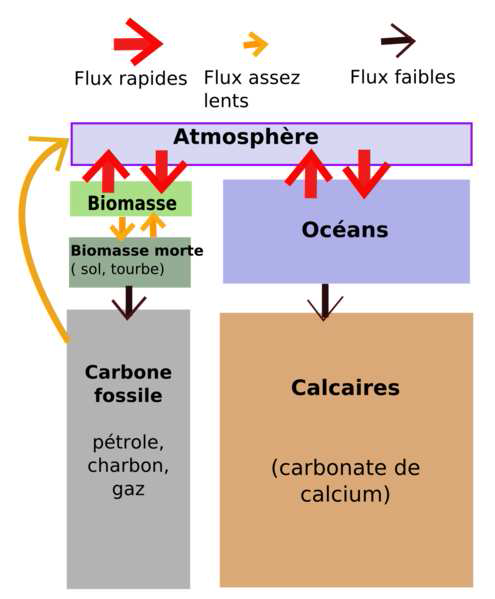
\includegraphics[scale=0.3]{images/cycle_carbone.png}
\begin{itemize}
	\item les flux rapides, susceptibles d’avoir des conséquences à court terme sur le climat (de la décennie à quelques siècles) ;
	\item les flux assez lents dont les conséquences ne s’observent que sur le moyen terme (quelques siècles) ;
	\item les flux très lents dont les conséquences ne s’observent que sur le très long terme (plusieurs millions d’années) : ces flux-là sont trop lents pour être à l’origine du récent changement climatique, et ne pourront pas équilibrer les rejets d’origine anthropiques.
\end{itemize}
\color{black}



\subsubsection{Qu'est-ce que l'ozone troposphérique ?}
\color{cyan}
L’ozone troposphérique est ce qu’on appelle un polluant secondaire, un photo-oxydant, formé par l’action du rayonnement solaire sur des polluants primaires précurseurs.

Il est le produit de réactions chimiques complexes faisant intervenir les oxydes d’azote, les composes organiques volatils, le monoxyde de carbone, la température et la lumière solaire. L’ozone troposphérique a un effet toxique sur les êtres humains et sur la végétation.
\color{black}



\subsubsection{Pourquoi il y a plus d'ozone troposphérique en milieu rural qu'en zone urbaine ?}
\color{cyan}
On retrouve l'ozone formé à partir de la pollution urbaine. Les polluants précurseurs étant en faible quantité, ils ne peuvent réduire les concentrations d'ozone la nuit. Les teneurs sont donc quasi-stationnaires.
\color{black}






\subsection{Decroly}



\subsubsection{Logique}
\begin{description}
	\item [Population de 25.000.000 sur Terre en l'an 0. ]
	\color{cyan}Faux\color{black}

	\item [Judéo-Chrétien n'a pas de valeurs sacrées aux éléments de la nature. ]
	\color{cyan}Vrai\color{black}

	\item [Modernisme est représentation de distance entre l'homme et la nature. ]
	\color{cyan}\color{black}

	\item [Fin 18ème, Anthoropocène. ]
	\color{cyan}Vrai\color{black}

	\item [Lula a voulu diminuer les productions de soja. ]
	\color{cyan}Faux\color{black}
	
	\item [Le pastoralisme décrit la relation interdépendante entre les éleveurs, leurs troupeaux et leur biotope. ]
	\color{cyan}Vrai\color{black}
	
	\item [La relation de pastoralisme existe depuis environ 10 000 ans. ]
	\color{cyan}Vrai\color{black}

	\item [Nord Sahel, extension de la culture pluviale au détriment du pastoralisme. ]
	\color{cyan}Vrai\color{black}

	\item [La finalité de l'agriculture au Sahel avant la colonisation est de faire un maximum de profit. ]
	\color{cyan}Faux\color{black}
	
	\item [La finalité de l'agriculture au Sahel avant la colonisation est d'avoir le plus d'homme sous son ordre. ]
	\color{cyan}Vrai\color{black}

	\item [Augmentation des prix agricoles au Niger entre 1950 et 1970. ]
	\color{cyan}Vrai\color{black}

	\item [40\% d'eau douce est amenée sur terre par l'évaporation des océans. ]
	\color{cyan}Vrai\color{black}
	
	\item [47\% d'eau douce est amenée sur terre par l'évaporation des écoulement des eaux vers la mer. ]
	\color{cyan}Vrai\color{black}
	
	\item [2,5\% d'eau douce est amenée sur terre par l'évaporation des fontes des glaces. ]
	\color{cyan}Vrai\color{black}

	\item [Projet de transfert d'eau en Tunisie au bénéfice du Tourisme. ]
	\color{cyan}Vrai\color{black}

	\item [GAP financé par les organismes d'aide au développement. ]
	\color{cyan}Faux\color{black}

	\item [GAP accompagné d'une réforme agraire pour les Kurdes. ]
	\color{cyan}Faux\color{black}

	\item [La Turquie considère eaux du Tigre et de l'Euphrate comme richesse naturelle nationale. ]
	\color{cyan}Vrai\color{black}

	\item [Reduction de la biodiversité plus rapide que rejets Pb. ]
	\color{cyan}Faux\color{black}

	\item [Dès 1910, la production de caoutchouc hollandaise a supplanté la production brésilienne. ]
	\color{cyan}Vrai\color{black}

	\item [La rouille su-américaine attaque plus les hévéas cultivés que les naturels. ]
	\color{cyan}Vrai\color{black}
\end{description}



\subsubsection{Définition : obsolescence}
\color{cyan}
\begin{description}
	\item [L'obsolescence] est le fait pour un produit d’être dépassé, et donc de perdre une partie de sa valeur en raison de la seule évolution technique (on parle alors d'\textbf{obsolescence technique}) ou de la mode (on utilise alors plutôt le mot "démodé") ;
	\item [L’obsolescence programmée] est le nom donné à l'ensemble des techniques visant à réduire la durée de vie ou d'utilisation d'un produit afin d'en augmenter le taux de remplacement.\color{black}
\end{description}
\color{black}



\subsubsection{Pourquoi les USA ont tellement de terres irriguées ?}
\color{cyan}
\color{black}



\subsubsection{Pourcentage d'agricultue en Israêl ? Quel est le secteur le plus exploité ?}
\color{cyan}
\color{black}



\subsubsection{Dans quel domaine la Turquie met toute son économie ?}
\color{cyan}
Dans le tourisme
\color{black}



\subsubsection{Question sur le pourcentage de forêt amazoniene déboisée}
\color{cyan}
\color{black}



\subsubsection{Question sur le pourcentage d'unités de conservation de la forêt brésilienne}
\color{cyan}
\color{black}



\subsubsection{Quelles sont les 3 motivations principales du développement de l'Amazonie et pourquoi il n'y a pas de réforme agraire ?}
\color{cyan}
\color{black}



\subsubsection{Pourquoi le Brésil a encouragé la déforestation et pourquoi il n'y a pas de réforme agraire}
\color{cyan}
Entre 1970 et 1990, la logique était un déboisement motivé par la spéculation foncière ; On achète des terres pour faire augmenter leur prix et ensuite on les revends. Dans les années '90, le déboisement était plutôt motivé par la rentabilité économique des productions de soja et de viande de boeuf ; On a besoin de place pour ces productions car la demande mondiale est élevée.
\color{black}



\subsubsection{Pourquoi le Brésil préfère une réforme agraire ?}
\color{cyan}
Coexistence de 2 partis : oligarchie foncière et bourgeoise cafétière
Les facteurs influençant ...
\begin{itemize}
	\item Motifs socioplitiques ;
	\item Motifs économiques ;
	\item Motifs stratégiques.
\end{itemize}
\color{black}